\documentclass[a4paper]{article}
\usepackage[fontset=fandol]{ctex}
\usepackage[margin=2cm]{geometry}
\usepackage{pdfpages}
\usepackage{hyperref}
\usepackage{longtable}
\title{CMU S11-751/18-781: Speech Recognition and Understanding (Fall 2023)}
\author{Codex harness-managed build from course page, public videos, and supplemental official materials}
\date{\today}
\begin{document}
\maketitle
\tableofcontents
\newpage
\section*{课程说明}
本教材按 harness-managed 流水线逐讲生成，并只纳入通过 evaluator gate 的章节。
\addcontentsline{toc}{section}{课程说明}
\section*{课程目录}
\addcontentsline{toc}{section}{课程目录}
\begin{longtable}{p{0.08\textwidth}p{0.55\textwidth}p{0.15\textwidth}p{0.15\textwidth}}
\textbf{讲次} & \textbf{主题} & \textbf{日期} & \textbf{状态}\\
\hline
01 & Course Overview & 2023-08-28 & deliverable\\
02 & Introduction of Speech Recognition & 2023-08-30 & deliverable\\
03 & Speech Recognition Formulations & 2023-09-06 & deliverable\\
04 & Feature Extraction & 2023-09-11 & deliverable\\
05 & Acoustic Model Overview & 2023-09-13 & deliverable\\
06 & Alignment Problems & 2023-09-18 & deliverable\\
07 & K-means, GMM, EM Algorithm & 2023-09-20 & deliverable\\
08 & Forward-Backward Algorithm for HMM & 2023-09-25 & deliverable\\
09 & Forward-Backward Algorithm for HMM & 2023-09-27 & deliverable\\
10 & Forward-Backward Algorithm for CTC and Viterbi Algorithm & 2023-10-02 & deliverable\\
11 & N-gram Language Models & 2023-10-02 & deliverable\\
12 & Search & 2023-10-11 & deliverable\\
13 & ESPnet Hands-on Tutorial I & 2023-10-23 & deliverable\\
14 & ESPnet Hands-on Tutorial II & 2023-10-25 & deliverable\\
15 & Deep Neural Network for Acoustic Modeling & 2023-10-30 & deliverable\\
16 & Neural Network Language Model & 2023-11-01 & deliverable\\
17 & End-to-End ASR: Attention & 2023-11-06 & deliverable\\
18 & End-to-End ASR: CTC & 2023-11-08 & deliverable\\
19 & End-to-End ASR: RNN-T & 2023-11-13 & deliverable\\
20 & Advanced Topics on End-to-End ASR I & 2023-11-15 & deliverable\\
21 & Advanced Topics on End-to-End ASR II & 2023-11-20 & deliverable\\
22 & Guest Lecture I & 2023-11-27 & deliverable\\
23 & Guest Lecture II & 2023-11-29 & deliverable\\
\end{longtable}

\section*{来源说明}
\addcontentsline{toc}{section}{来源说明}
本书以 2023 年课程页与官方公开录像为主；当某讲在 2023 年没有公开视频时，才使用同门课同主题的官方公开辅助材料或明确标注的官方重建材料。
\begin{longtable}{p{0.08\textwidth}p{0.32\textwidth}p{0.18\textwidth}p{0.34\textwidth}}
\textbf{讲次} & \textbf{主题} & \textbf{来源类型} & \textbf{说明}\\
\hline
01 & Course Overview & official auxiliary video & Reconstructed from the 2023 course row plus an official same-course auxiliary public video.\\
02 & Introduction of Speech Recognition & 2023 official video & Directly grounded in the official Fall 2023 WAVLab public playlist.\\
03 & Speech Recognition Formulations & 2023 official video & Directly grounded in the official Fall 2023 WAVLab public playlist.\\
04 & Feature Extraction & 2023 official video & Directly grounded in the official Fall 2023 WAVLab public playlist.\\
05 & Acoustic Model Overview & official auxiliary video & Reconstructed from the 2023 course row plus an official same-course auxiliary public video.\\
06 & Alignment Problems & 2023 official video & Directly grounded in the official Fall 2023 WAVLab public playlist.\\
07 & K-means, GMM, EM Algorithm & 2023 official video & Directly grounded in the official Fall 2023 WAVLab public playlist.\\
08 & Forward-Backward Algorithm for HMM & 2023 official video & Directly grounded in the official Fall 2023 WAVLab public playlist.\\
09 & Forward-Backward Algorithm for HMM & 2023 official video & Directly grounded in the official Fall 2023 WAVLab public playlist.\\
10 & Forward-Backward Algorithm for CTC and Viterbi Algorithm & 2023 official video & Directly grounded in the official Fall 2023 WAVLab public playlist.\\
11 & N-gram Language Models & 2023 official video & Directly grounded in the official Fall 2023 WAVLab public playlist.\\
12 & Search & 2023 official video & Directly grounded in the official Fall 2023 WAVLab public playlist.\\
13 & ESPnet Hands-on Tutorial I & official auxiliary video & Reconstructed from the 2023 course row plus an official same-course auxiliary public video.\\
14 & ESPnet Hands-on Tutorial II & official auxiliary video & Reconstructed from the 2023 course row plus an official same-course auxiliary public video.\\
15 & Deep Neural Network for Acoustic Modeling & 2023 official video & Directly grounded in the official Fall 2023 WAVLab public playlist.\\
16 & Neural Network Language Model & 2023 official video & Directly grounded in the official Fall 2023 WAVLab public playlist.\\
17 & End-to-End ASR: Attention & 2023 official video & Directly grounded in the official Fall 2023 WAVLab public playlist.\\
18 & End-to-End ASR: CTC & 2023 official video & Directly grounded in the official Fall 2023 WAVLab public playlist.\\
19 & End-to-End ASR: RNN-T & 2023 official video & Directly grounded in the official Fall 2023 WAVLab public playlist.\\
20 & Advanced Topics on End-to-End ASR I & 2023 official video & Directly grounded in the official Fall 2023 WAVLab public playlist.\\
21 & Advanced Topics on End-to-End ASR II & 2023 official video & Directly grounded in the official Fall 2023 WAVLab public playlist.\\
22 & Guest Lecture I & official reconstruction & Reconstructed from official course-page rows and other official public materials without a recovered lecture video.\\
23 & Guest Lecture II & official reconstruction & Reconstructed from official course-page rows and other official public materials without a recovered lecture video.\\
\end{longtable}

\section{Course Overview}

\includepdf[pages=-,pagecommand={\thispagestyle{plain}}]{../lectures/01_course_overview/lecture_01_note.pdf}

\section{Introduction of Speech Recognition}

\includepdf[pages=-,pagecommand={\thispagestyle{plain}}]{../lectures/02_introduction_of_speech_recognition/lecture_02_note.pdf}

\section{Speech Recognition Formulations}

\includepdf[pages=-,pagecommand={\thispagestyle{plain}}]{../lectures/03_speech_recognition_formulations/lecture_03_note.pdf}

\section{Feature Extraction}

\includepdf[pages=-,pagecommand={\thispagestyle{plain}}]{../lectures/04_feature_extraction/lecture_04_note.pdf}

\section{Acoustic Model Overview}

\includepdf[pages=-,pagecommand={\thispagestyle{plain}}]{../lectures/05_acoustic_model_overview/lecture_05_note.pdf}

\section{Alignment Problems}

\includepdf[pages=-,pagecommand={\thispagestyle{plain}}]{../lectures/06_alignment_problems/lecture_06_note.pdf}

\section{K-means, GMM, EM Algorithm}

\includepdf[pages=-,pagecommand={\thispagestyle{plain}}]{../lectures/07_kmeans_gmm_em_algorithm/lecture_07_note.pdf}

\section{Forward-Backward Algorithm for HMM}

\includepdf[pages=-,pagecommand={\thispagestyle{plain}}]{../lectures/08_forward_backward_hmm_i/lecture_08_note.pdf}

\section{Forward-Backward Algorithm for HMM}

\includepdf[pages=-,pagecommand={\thispagestyle{plain}}]{../lectures/09_forward_backward_hmm_ii/lecture_09_note.pdf}

\section{Forward-Backward Algorithm for CTC and Viterbi Algorithm}

\includepdf[pages=-,pagecommand={\thispagestyle{plain}}]{../lectures/10_forward_backward_ctc_viterbi/lecture_10_note.pdf}

\section{N-gram Language Models}

\includepdf[pages=-,pagecommand={\thispagestyle{plain}}]{../lectures/11_ngram_language_models/lecture_11_note.pdf}

\section{Search}

\includepdf[pages=-,pagecommand={\thispagestyle{plain}}]{../lectures/12_search/lecture_12_note.pdf}

\section{ESPnet Hands-on Tutorial I}

\includepdf[pages=-,pagecommand={\thispagestyle{plain}}]{../lectures/13_espnet_hands_on_i/lecture_13_note.pdf}

\section{ESPnet Hands-on Tutorial II}

\includepdf[pages=-,pagecommand={\thispagestyle{plain}}]{../lectures/14_espnet_hands_on_ii/lecture_14_note.pdf}

\section{Deep Neural Network for Acoustic Modeling}

\includepdf[pages=-,pagecommand={\thispagestyle{plain}}]{../lectures/15_dnn_for_acoustic_modeling/lecture_15_note.pdf}

\section{Neural Network Language Model}

\includepdf[pages=-,pagecommand={\thispagestyle{plain}}]{../lectures/16_neural_network_language_model/lecture_16_note.pdf}

\section{End-to-End ASR: Attention}

\includepdf[pages=-,pagecommand={\thispagestyle{plain}}]{../lectures/17_end_to_end_asr_attention/lecture_17_note.pdf}

\section{End-to-End ASR: CTC}

\includepdf[pages=-,pagecommand={\thispagestyle{plain}}]{../lectures/18_end_to_end_asr_ctc/lecture_18_note.pdf}

\section{End-to-End ASR: RNN-T}

\includepdf[pages=-,pagecommand={\thispagestyle{plain}}]{../lectures/19_end_to_end_asr_rnnt/lecture_19_note.pdf}

\section{Advanced Topics on End-to-End ASR I}
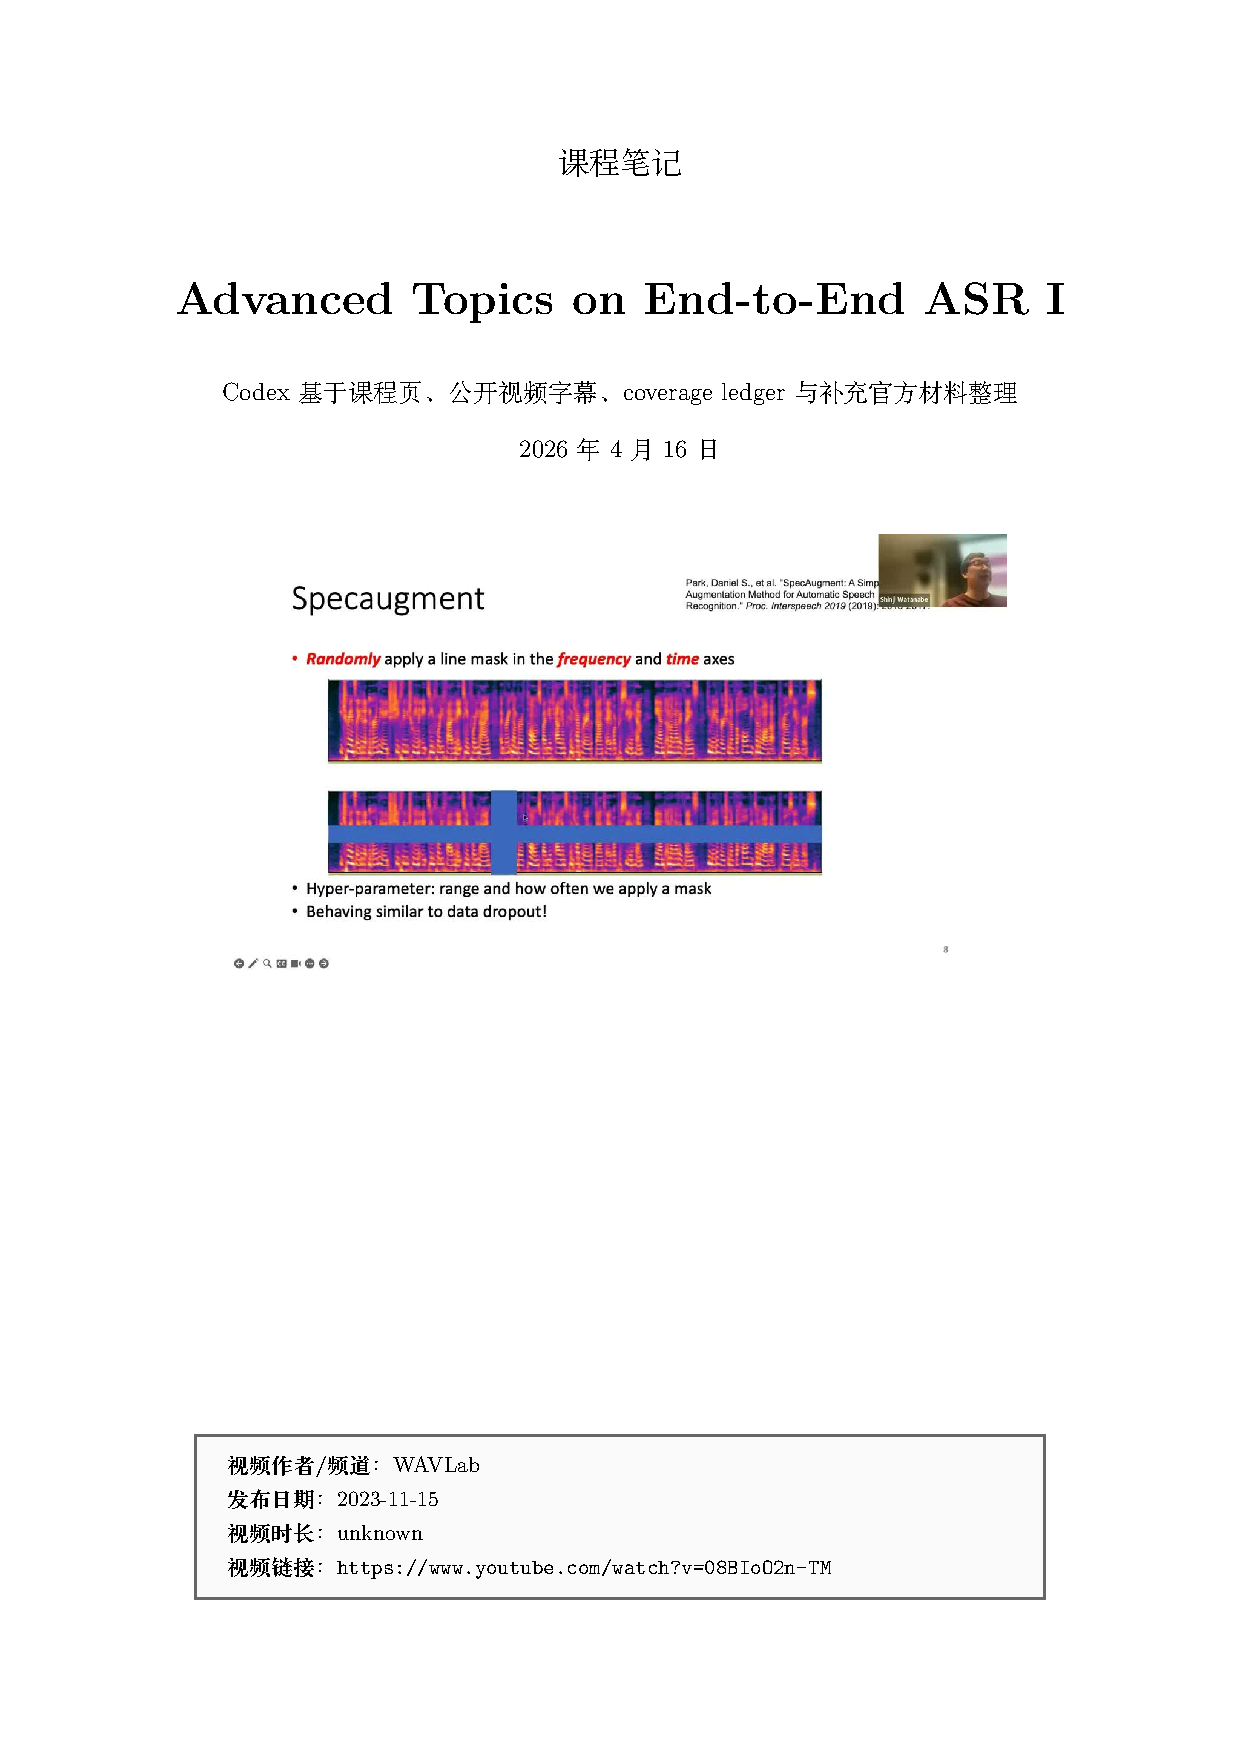
\includepdf[pages=-,pagecommand={\thispagestyle{plain}}]{../lectures/20_advanced_topics_on_end_to_end_asr_i/lecture_20_note.pdf}

\section{Advanced Topics on End-to-End ASR II}
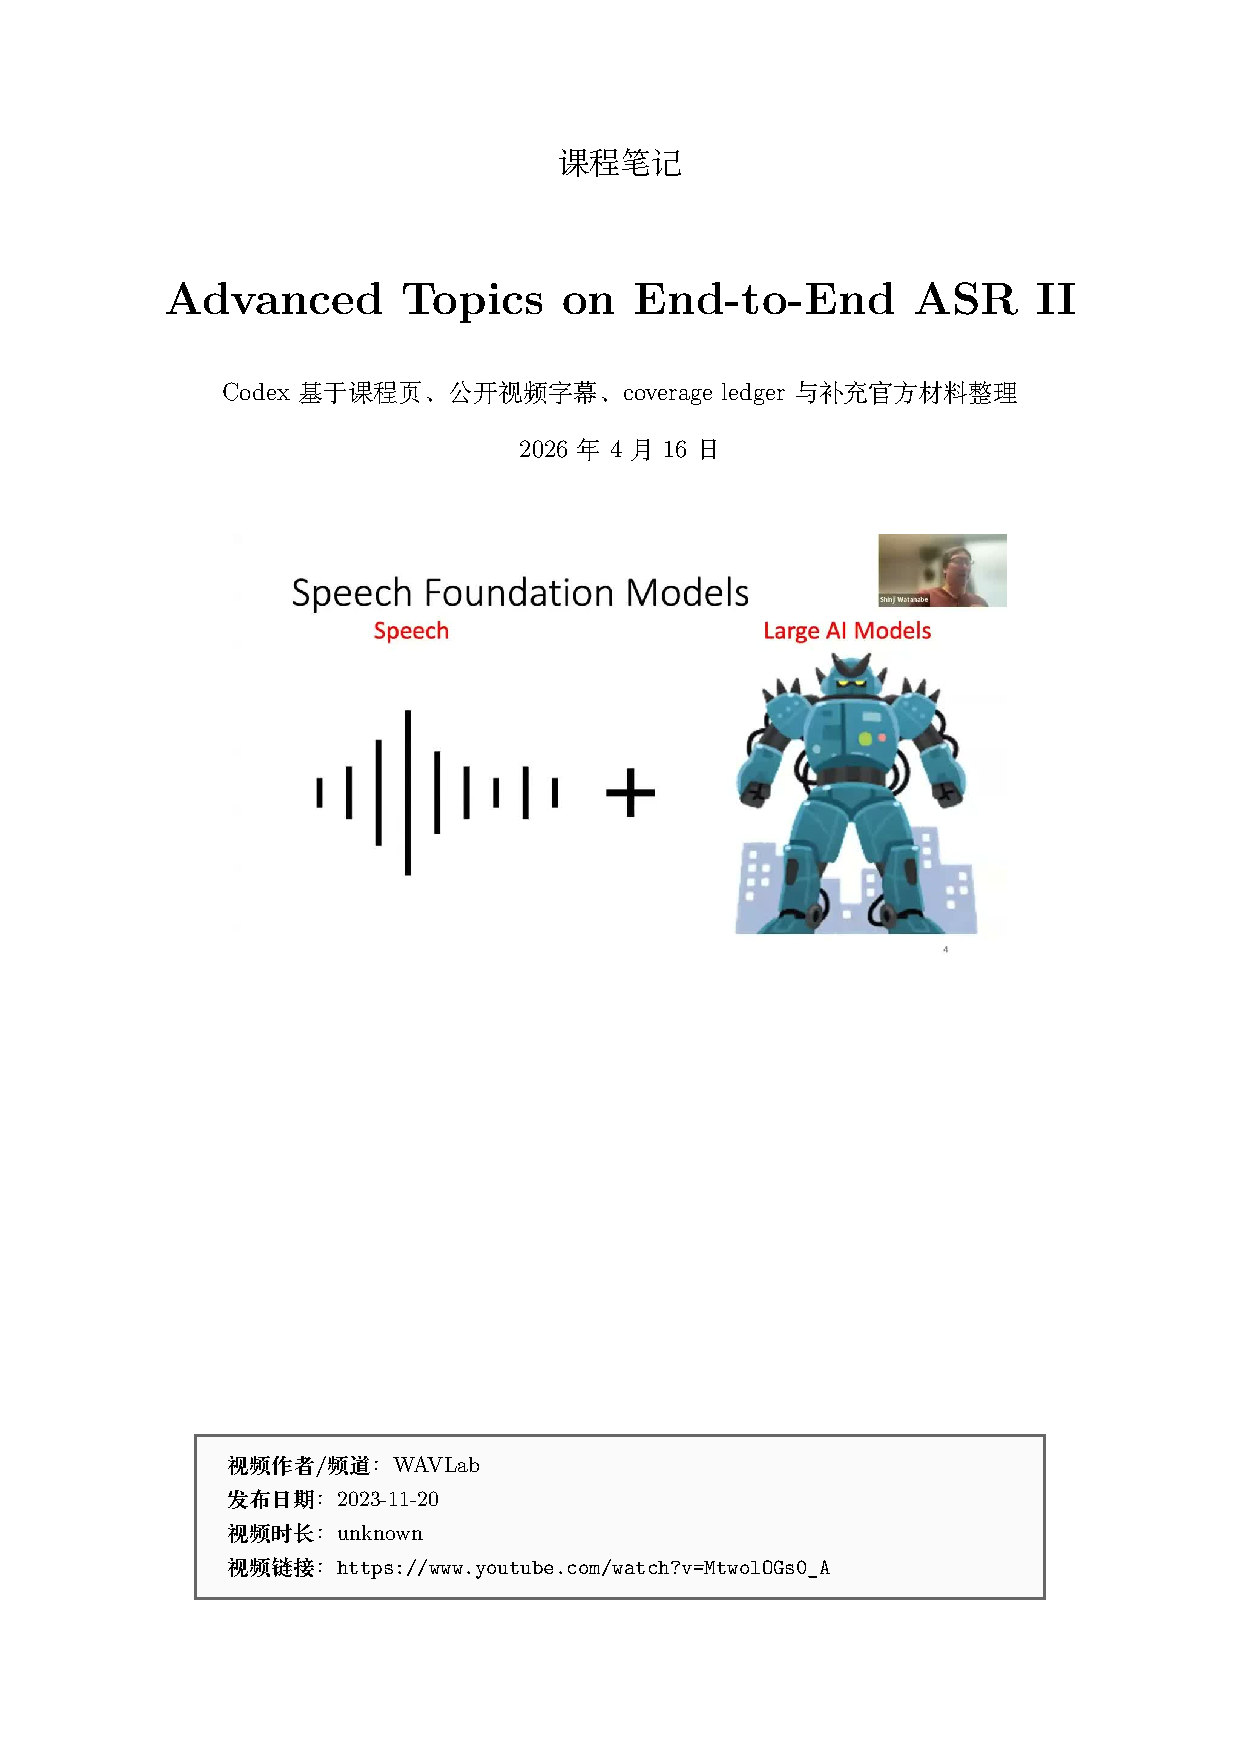
\includepdf[pages=-,pagecommand={\thispagestyle{plain}}]{../lectures/21_advanced_topics_on_end_to_end_asr_ii/lecture_21_note.pdf}

\section{Guest Lecture I}
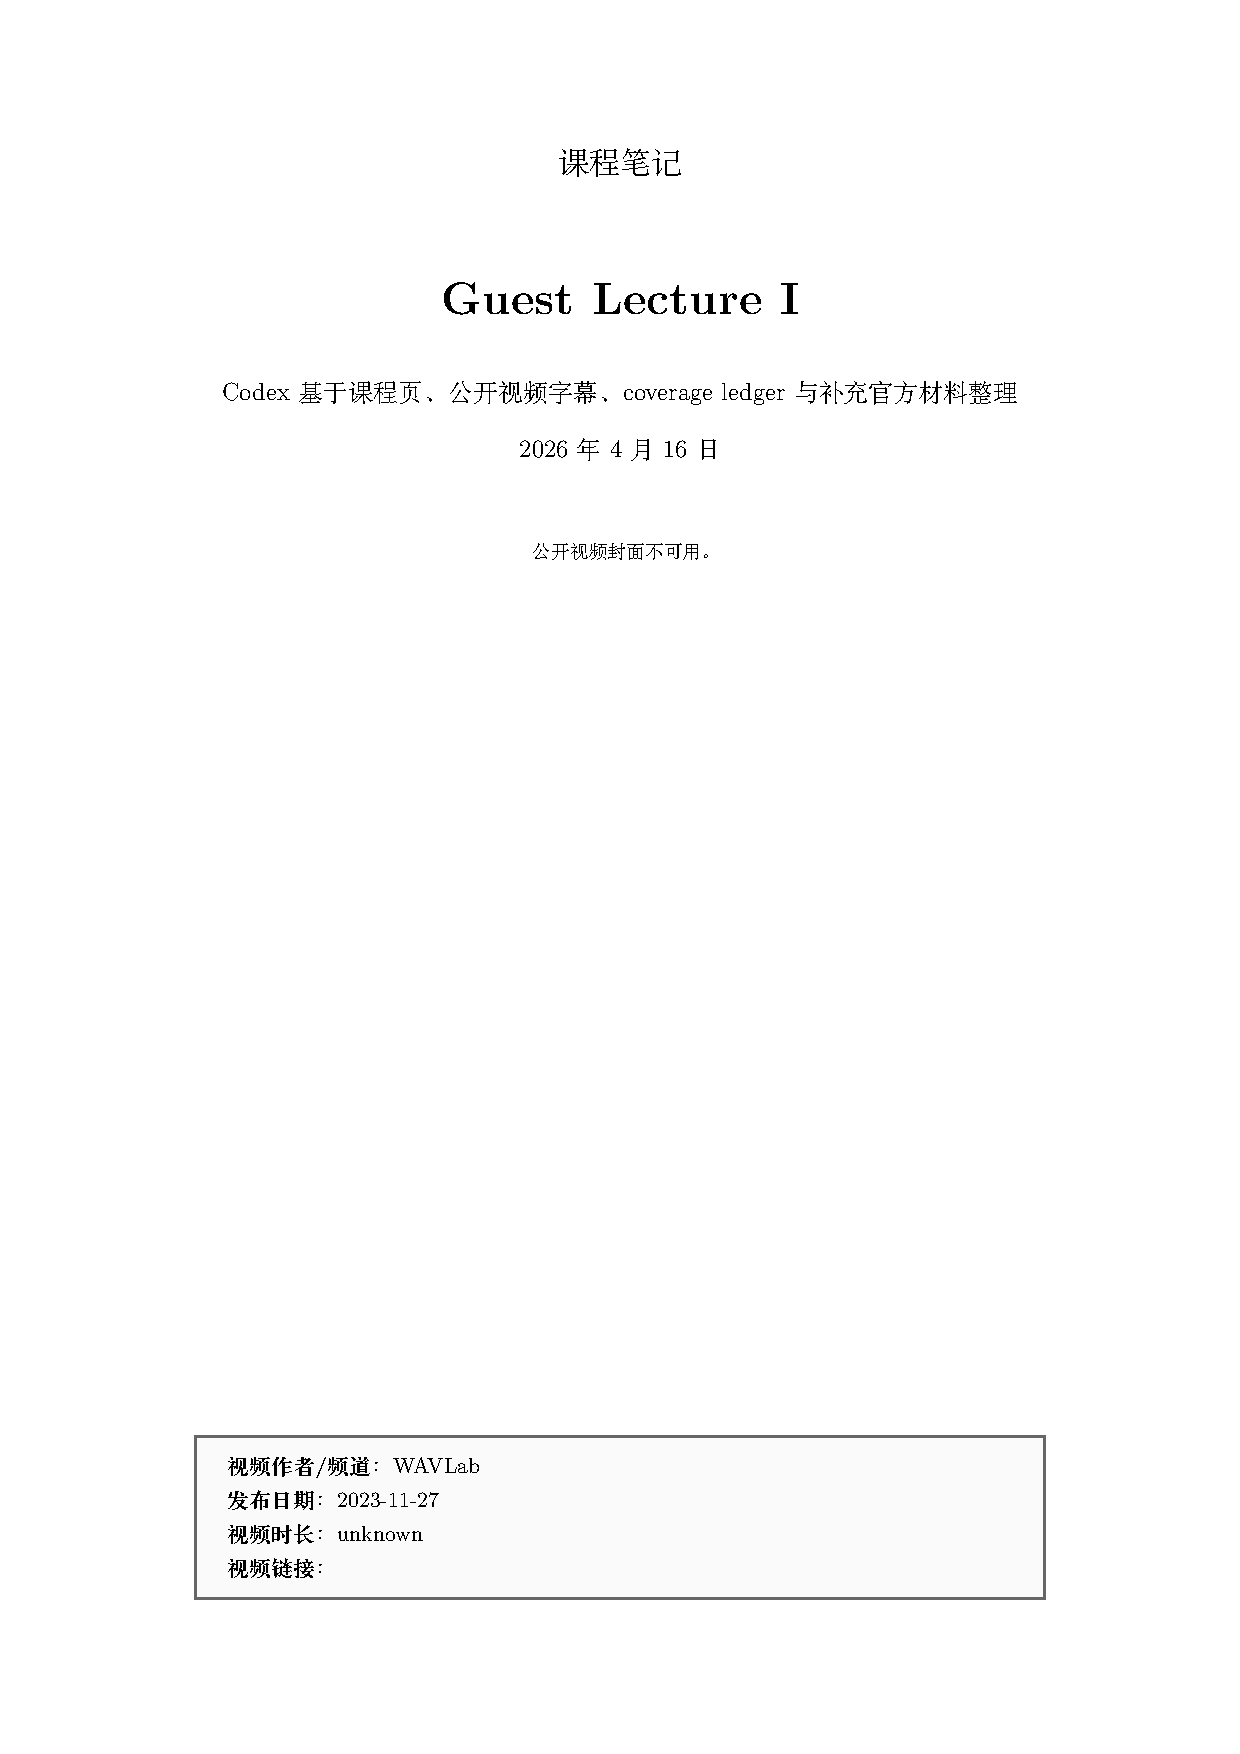
\includepdf[pages=-,pagecommand={\thispagestyle{plain}}]{../lectures/22_guest_lecture_i/lecture_22_note.pdf}

\section{Guest Lecture II}
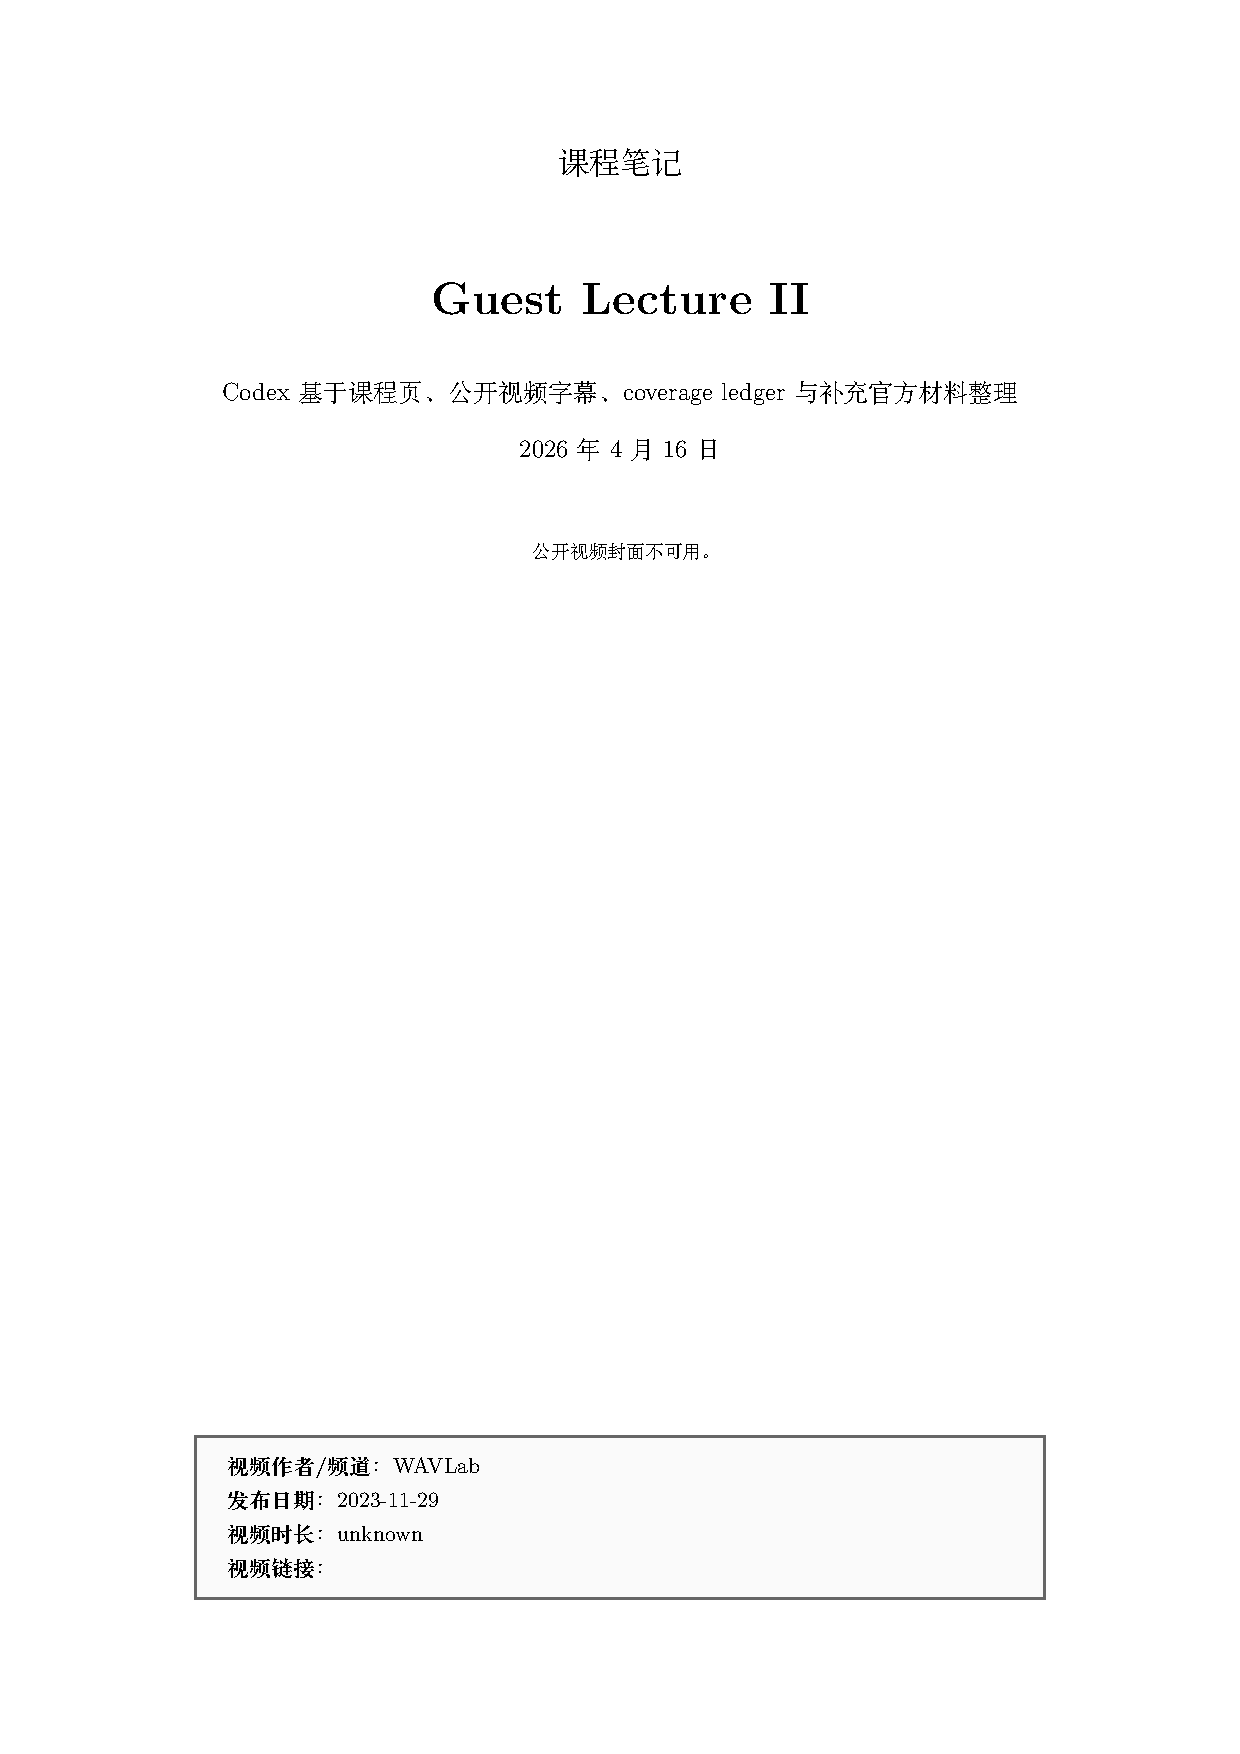
\includepdf[pages=-,pagecommand={\thispagestyle{plain}}]{../lectures/23_guest_lecture_ii/lecture_23_note.pdf}

\end{document}
